\section{Enantiomorphing chiral crosses}\label{sec:results:EnantiomorphingChiralCrosses}
This section has largely been copied verbatum from the manuscript \textit{``Enantiomorphing Chiral Plasmonic Nanostructures: A Counterintuitive Sign Reversal of the Nonlinear Circular Dichroism''}, Joel~T.~Collins et. al. \cite{Collins2018}. 
Experiments were planned by V. K. Valev. Samples were prepared by N. V. S. Braz and P. A. Warburton. Experiments were executed by V. K. Valev, E. Slenders and M. Ameloot. Near-field and scattering simulations were performed by X. Zheng and G. A. E. Vandenbosch. Numerical simulations of the far-field, linear CD were performed by S. Zu and Z. Fang. 
Analysis of the nonlinear microscopy data was performed by myself, with Python code including sections written by V. K. Valev. The formulation and analysis of modal circular-dichroism based on the near-field simulations was also performed by myself. I produced the first draft of the manuscript, and all authors have subsiquently contributed. 
\\

Plasmonic nanostructures have demonstrated a remarkable ability to control light in ways never observed in nature, as the optical response is closely linked to their flexible geometric design.
Due to lack of mirror symmetry, chiral nanostructures allow twisted electric field “hotspots” to form at the material surface. 
These hotspots depend strongly on the optical wavelength and nanostructure geometry.
Understanding the properties of these chiral hotspots is crucial for their applications; for instance, in enhancing the optical interactions with chiral molecules. 
Here, the results of an elegant experiment are presented: by designing 35 intermediate geometries, the structure is “enantiomorphed” from one handedness to the other, passing through an achiral geometry. 
Nonlinear multiphoton microscopy is used to demonstrate a new kind of double-bisignate circular dichroism due to enantiomorphing, rather than wavelength change.
From group theory, a fundamental origin of this plasmonic chiroptical response is proposed. The analysis allows the optimization of plasmonic chiroptical materials.

\subsection{Introduction}\label{sec:results:EnantiomorphingChiralCrosses:introduction}
Throughout the 19th and most of the 20th century, chirality has been associated with chemistry. However, whereas chirality can be crucial for understanding molecules, molecules are not best suited for understanding chirality. Indeed, there are various forms of chirality, such as helical chirality, propeller chirality, supramolecular chirality, extrinsic chirality, etc.\cite{Collins2017, Valev2013b}. These forms all depend on chirality parameters. 
Ideally, we would like to be able to vary these parameters, i.e., to follow the parameter values as chiral systems transition from one chiral form into another. However, it is impossible to control the size of atoms, the length of chemical bonds, and the orientation of orbitals. Modern nanofabrication techniques have lifted the limitations on tuning chiral parameters.

Using modern nanofabrication methods, it is possible to explore the evolution of chiral forms, by preparing numerous intermediate geometries. This is important because it opens the possibility to tune and optimize the chirality parameters, which enable interesting properties. For instance, by maximizing the geometric chirality parameter, it is possible to achieve negative refractive index materials \cite{Pendry2004a}. Such materials could lead to super-lenses \cite{Khorasaninejad2016}, and various applications that depend on the control of circularly polarized light (CPL). In turn, CPL could find applications in spintronics \cite{Farshchi2011b} and quantum computing \cite{Wagenknecht2010a, Sherson2006a}.
Moreover, by optimizing a parameter called \textit{optical chirality} \cite{Tang2010} it has been shown that “superchiral” light configurations can be achieved. In such configurations, the pitch of the electric field of light is shorter than that of circularly polarized light, thereby enabling stronger chiroptical effects \cite{Hendry2010, Hendry2012, Tullius2015}. Importantly, optical chirality is particularly enhanced at the surface of chiral plasmonic nanostructures \cite{Schaferling2012, Karimullah2015}, resulting in large enhancements in measurable circular dichroism (CD) \cite{Maoz2013, Wang2014c, Ma2013b, Zhang2013}.

Despite the advantages of creating intermediate geometries, it is rare to find studies where these have been investigated in detail. Between two enantiomorphs, there can be several path- ways for intermediate geometries and those might be quite different (Figure~\ref{fig:results:EnantiomorphingChiralCrosses:setup}a). 
Also, a priory, it is not clear what the best number of intermediate geometries should be. Indeed this is highly dependent on the geometric and material properties of the structures, as well as on the wavelength ranges used. In the literature, examples can be found of studying both enantio- morphs of a structure, its achiral variant, and a small number of intermediate steps only \cite{Zu2016}.Consequently, important and interesting behavior can go unnoticed.

\begin{figure}[htb!]	
    \centering	
    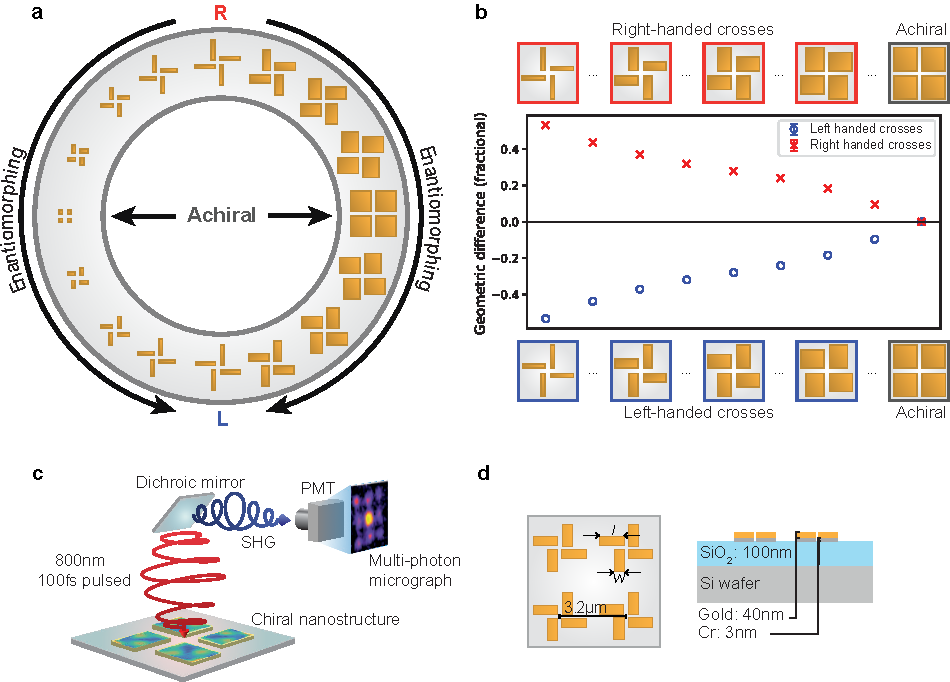
\includegraphics[scale=0.8]{./figures/results/EnantiomorphingChiralCrosses/setup.pdf}
    \caption{\label{fig:results:EnantiomorphingChiralCrosses:setup}
    \textbf{a)} Representation of two possible pathways to enantiomorph a right-handed structure (R) into a left-handed structure (L), through an achiral geometry. Here, we examine the pathway on the right side of the circle. \textbf{b)} As the left-handed chiral crosses change into achiral square structures and into right-handed chiral crosses, the chiral geometric difference diminishes until it reaches 0 in the achiral case and then reverse its value. \textbf{c)} Schematic diagram of the multiphoton microscopy experiments. \textbf{d)} Geometry and depth profile of the chiral crosses samples.}	
\end{figure}

Here, we report an elegant experiment, impossible to per-
form with chiral molecules: by designing 35 intermediate geometries, we ``enantiomorph'' plasmonic nanostructures from one handedness to the other, passing through an achiral geometry. 
We demonstrate a new kind of bisignate (of two signs) CD due to enantiomorphing, rather than wavelength change, in the nonlinear emission from near-field hotspots. Contrary to what would be expected from pure geometric considerations, the nonlinear chiroptical signal reverses sign thrice, i.e., it is double-bisignate. In order to understand this result, we perform a full modal analysis of the structures in combination with irreducible representations (group theory). 
Interestingly, we find that, regardless of their handedness, chiral nanostructures contain modes that can be excited by both left and right circularly polarized (LCP and RCP) light. Furthermore, which modes are dominant (i.e., couple strongest to light) depends on the wavelength or the shape/dimensions of the nanostructure. It is therefore perfectly possible to engineer chiral nano- materials that, at a given wavelength, can only be excited with the “wrong” kind of CPL. 
Our findings offer the possibility of tuning chiroptical response by selecting particular electromagnetic modes, or sets of modes, among hundreds available, which can enable much more sensitive chiroptical control than what is currently available.

\subsection{Results}\label{sec:results:EnantiomorphingChiralCrosses:results}

We begin by presenting the purely geometric considerations. Starting with left-handed crosses, we morph their geometry in discrete steps, first into achiral squares and then into right-handed chiral crosses (Figure~\ref{fig:results:EnantiomorphingChiralCrosses:setup}b). For the purposes of comparison, we use a measure of ``chiral geometric difference'' (not to be confused with the geometric chirality parameter). 
% TODO: Write up the geometric difference stuff in appendix
This quantity describes the area of maximal overlap that can be achieved between left- and right-handed structures, by rotating and translating the two mirror-image shapes, relative to each other (\emph{\color{red}APPENDIX SECTION}). 
As Figure~\ref{fig:results:EnantiomorphingChiralCrosses:setup}b shows, the chiral geometric difference diminishes until it reaches 0, in the achiral case. However, the chiroptical properties of nanostructures depend on more than geometry alone; without considering material effects, and the properties of the incident light, no direct connection can be made between chiral geometric difference and chiroptical effects. This measure of chirality is in stark contrast to the double-bisignate response found in our nonlinear CD measurements.

For our experiments, we made use of multiphoton microscopy performed with CPL illumination at 800 nm and schematized in Figure~\ref{fig:results:EnantiomorphingChiralCrosses:setup}c. The instrument was a standard commercial model (the same as in our previous works \cite{Valev2012a}).
The collected light consisted mostly of the second harmonic generation (SHG). Specifically, a bandpass filter allowing 390 nm to 465 nm light was used and, although this filter passes a small part of two-photon luminescence signal, the SHG signal is clearly dominant in this spectral range. Since these nonlinear optical processes are enhanced in the regions of strong local field, \cite{Wang2013, Chen1983} they act as a sensitive far-field probe for local field effects. 

The samples are chiral crosses made of Au, deposited by electron beam lithography (EBL) on a Si substrate with a thermal oxide layer, and whose dimensions and depth profile are given in Figure~\ref{fig:results:EnantiomorphingChiralCrosses:setup}d. Each cross is composed of four separate nanostripes, with varying width $w$ and length $l$. The separation distance between nanostripes, at the centre of the crosses, is constant at $200\si{\nano\meter}$. The crosses are arranged in a $40 \times 40 \si{\micro\meter\squared}$ square array, with the distance between cross centres also kept constant at $3.2 \si{\micro\meter}$. 

\begin{figure}[htb!]	
    \centering	
    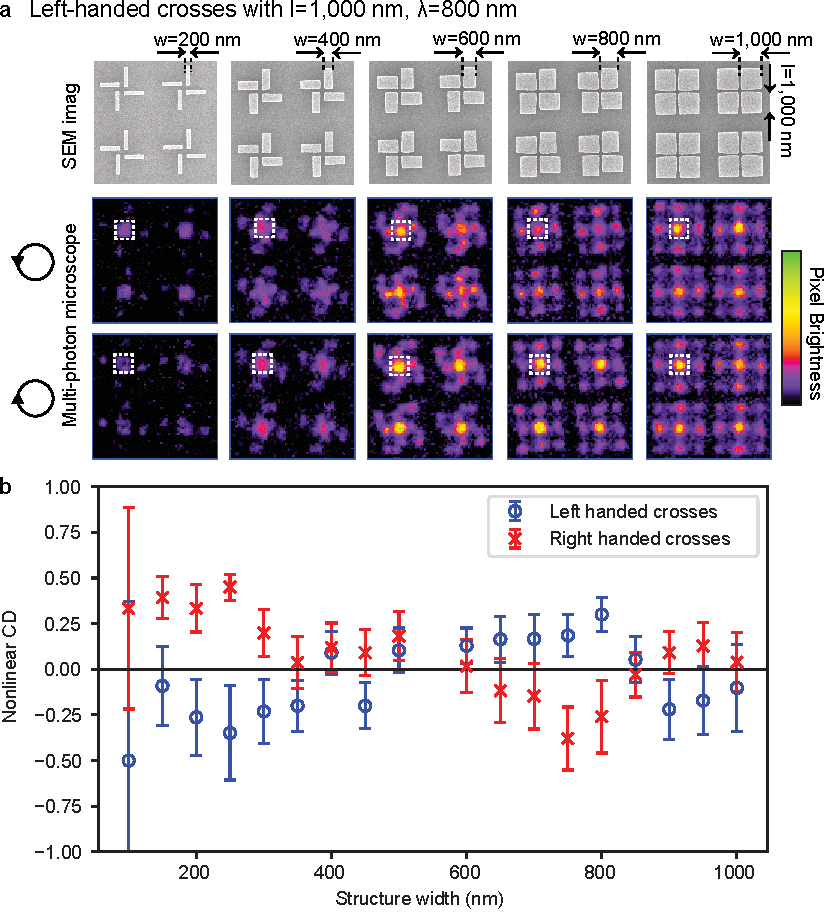
\includegraphics[scale=0.8]{./figures/results/EnantiomorphingChiralCrosses/l1000data.pdf}
    \caption{\label{fig:results:EnantiomorphingChiralCrosses:l1000data}
    Varying arm width of the nanostructure features at fixed l=1000nm. SEM images of 4 structure cells for each geometry \textbf{(a top)}, and SHG microscopy images \textbf{(a, lower)} under illumination from left and right circularly polarized light, at $800 \si{\nano\meter}$ wavelength. Scale (right) corresponds to image pixel brightness. \textbf{b)} Measured total nonlinear CD under $800 \si{\nano\meter}$ wavelength light is then calculated for each geometry. Our experiments reveal a counter-intuitive behavior for the second-harmonic generation circular dichroism (SHG-CD) – both the 0 value and the reversal occur before reaching the achiral geometry.}	
\end{figure}

Figure~\ref{fig:results:EnantiomorphingChiralCrosses:l1000data}a shows scanning electron microscopy (SEM) images of sample arrays. In these arrays, the length of the nanostripes is fixed ($1000 \si{\nano\meter}$) and the width changes from $200 \si{\nano\meter}$ to $1000 \si{\nano\meter}$ in steps of $200 \si{\nano\meter}$. Underneath each SEM are two corresponding multi-photon micrographs, obtained with LCP and RCP. The multi-photon microscopy images are color-coded for intensity and they show bright hotspots at the center of the chiral crosses (indicated with dashed-line squares for clarity). 
Similar hotspots have previously been observed at the center of G-shaped \cite{Valev2009a} and S-shaped \cite{Valev2014} nanostructured arrays. 
The hotspots correspond to a chiral coupling at the center of the unit cells that depends on the chirality of the nanostructures and the direction of CPL \cite{ Valev2014, Petralli-Mallow1993, Byers1994}. This dependence is expressed as a directly observable nonlinear CD effect (brightness of the hotspots, depending on the direction of CPL). Interestingly though, in this set of samples, the nonlinear CD changes sign between the chiral crosses with nanostripe width  $200 \si{\nano\meter}$ and $600 \si{\nano\meter}$, even though the structures have the same handedness.

The nonlinear CD reversal can be seen more quantitatively in Figure~\ref{fig:results:EnantiomorphingChiralCrosses:l1000data}b. Here, the nonlinear CD is obtained from the detected light upon LCR or RCP illumination according to 
$(I_{RCP}^{MP}-I_{LCP}^{MP})/(I_{RCP}^{MP}+I_{LCP}^{MP})$. The individual multi-photon intensity terms $I_{RCP}^{MP}$ and $I_{LCP}^{MP}$ were obtained from the pixel intensity at the center of the chiral crosses, where the chiral coupling is maximum and the characteristic response is most pronounced. For each chiral cross, the central hotspot intensity was averaged over 25 pixels (pixel array at $0.09\si{\micro\meter}$ per pixel). 
To account for individual variation between crosses, $I_{RCP}^{MP}$ and $I_{LCP}^{MP}$ were each obtained from further averaging the hotspots of 25 individual crosses. 
The error bars in Figure~\ref{fig:results:EnantiomorphingChiralCrosses:l1000data}b correspond to the standard deviation from this averaging. 
It should also be noted that the SEM pictures in Figure~\ref{fig:results:EnantiomorphingChiralCrosses:l1000data}a are only a subset of the entire range of samples we studied. The full set started from $w=100 \si{\nano\meter}$ and progressed to $w=1000 \si{\nano\meter}$, in steps of $50 \si{\nano\meter}$. 
Upon considering the nonlinear CD from all these samples, it is obvious that between $w=200 \si{\nano\meter}$ and $w=800 \si{\nano\meter}$, the chiroptical response is unambiguously reversed, i.e. with clearly separated error bars. The nonlinear CD that we measured is collected in the far-field and it is very different from the linear CD in far-field. 

In the far-field, the linear CD response is demonstrated by FDTD simulations data that are displayed in Figure~\ref{fig:results:EnantiomorphingChiralCrosses:l1000modes}a (further supporting data are provided in Figure S2 \emph{\color{red}APPENDIX SECTION} and Figure S3 \emph{\color{red}APPENDIX SECTION}). Clearly, the data in Figure~\ref{fig:results:EnantiomorphingChiralCrosses:l1000modes}a do not match those in Figure~\ref{fig:results:EnantiomorphingChiralCrosses:l1000data}b. One reason for this difference is that the nonlinear CD originates in the near-field, which is very different from the far-field in this kind of structures. To understand the observed reversal of the nonlinear CD, we need to examine the electromagnetic behaviour at the surface of the nanostructures. 

\subsection{Analysis and Discussion}\label{sec:results:EnantiomorphingChiralCrosses:discussion}

\noindent\textbf{To-do:}
\begin{itemize}
    \item Simple, plain English version of modal analysis and group theory.
    \item Lead from simple version of degenerate modes into main analysis.
\end{itemize}

\begin{figure}[htb!]	
    \centering	
    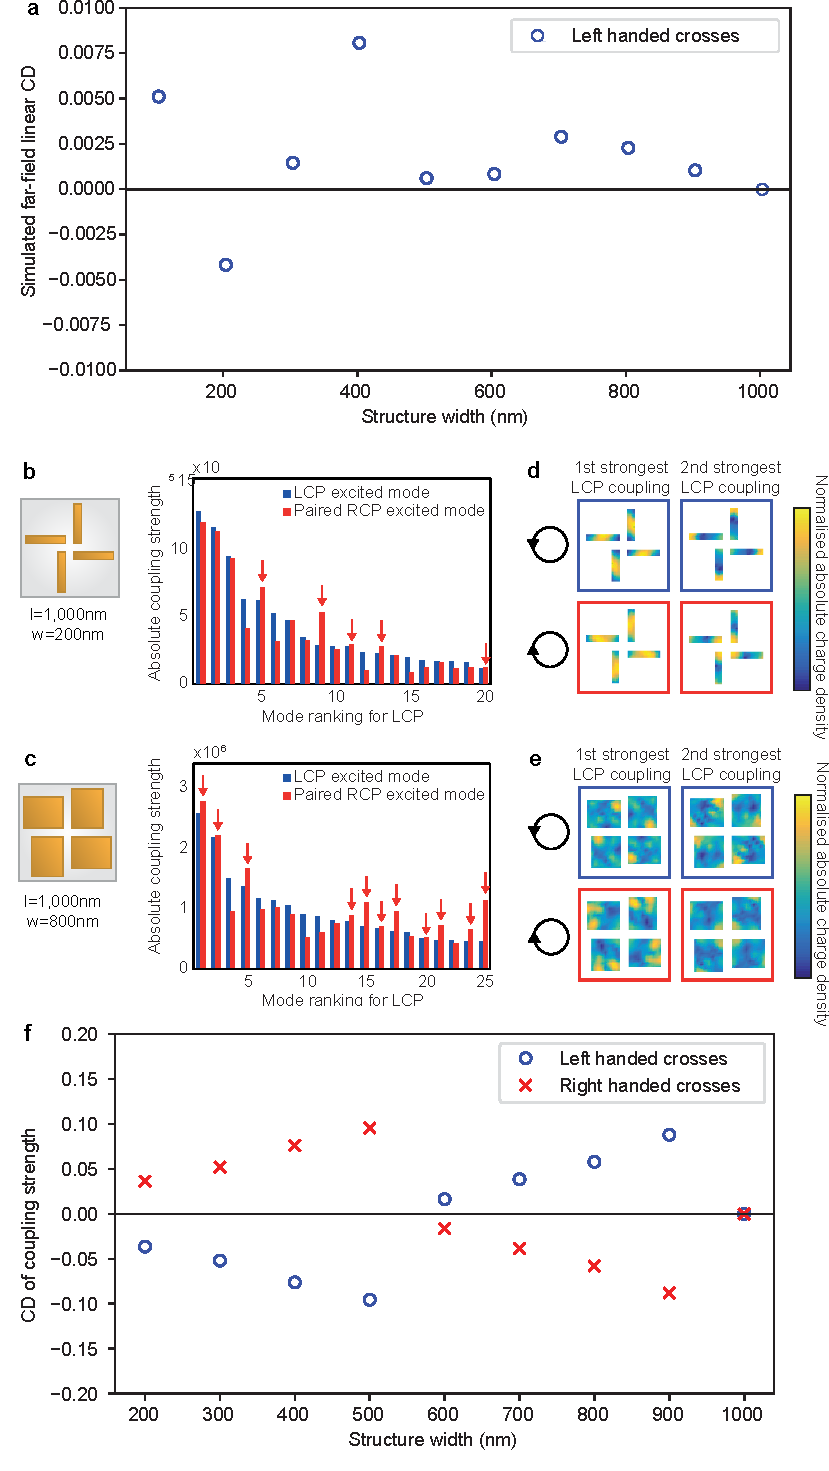
\includegraphics[scale=0.8]{./figures/results/EnantiomorphingChiralCrosses/l1000modes.pdf}
    \caption{\label{fig:results:EnantiomorphingChiralCrosses:l1000modes}
    \textbf{a.} Numerically-obtained far-field linear reflection CD for left-handed chiral cross structures. The lineshape of the linear CD response is significantly different to that obtained from nonlinear CD measurements. \textbf{b-f}. Simulation results showing modal composition of chiroptical response. Modal analysis of structures with arm length 1000nm, width 200nm \textbf{(b)} and 800nm \textbf{(c)}. The most LCP-dominant modes for each structure are plotted showing both LCP coupling strength (blue) and the correlated-mode RCP coupling strength (red). Modes coupling stronger to RCP than LCP are marked with arrows. Examples of individual modes (normalized absolute charge density) are shown for width 200nm \textbf{(d)} and 800nm \textbf{(e)}. The total coupling strength CD as defined in equation~\ref{eq:background:ChiropticalEffects:couplingCD} is plotted for varying arm width, at fixed $l=1000\si{\nano\meter}$ under $800\si{\nano\meter}$ wavelength light \textbf{(f)}.}	
\end{figure}

\begin{equation}\label{eq:background:ChiropticalEffects:couplingCD}	
	CD^{(Local)} \propto \frac{{\left\| {{c_n}^R(\omega )} \right\|}^2 - {\left\| {{c_n}^L(\omega )} \right\|}^2}{{\left\| {{c_n}^R(\omega )} \right\|}^2 + {\left\| {{c_n}^L(\omega )} \right\|}^2}
\end{equation}

